\documentclass[10pt,handout,compress]{beamer}
%\documentclass[10pt]{beamer}
%\documentclass[10pt,handout]{beamer}
%% Class options include: notes, notesonly, handout, trans,
%%                        hidesubsections, shadesubsections,
%%                        inrow, blue, red, grey, brown
%
%% Theme for beamer presentation.
\usepackage{beamerthemesplit}
\usepackage{natbib}    %number and author-year style referencing

\usepackage{times,epsfig,makeidx,amsfonts,amsmath,dcolumn,enumerate,multirow,graphicx,amssymb,colortbl,bm,pifont,color}
\usepackage[]{graphicx}
\usepackage{scalerel,amsfonts,bm}

\usepackage{xcolor}
\usepackage{hyperref}
\hypersetup{colorlinks=true,linkcolor=blue,urlcolor=blue}
\usepackage{listings}
\usepackage{fontawesome}


\newcommand*{\Scale}[2][4]{\scalebox{#1}{$#2$}}%
\setbeamertemplate{footline}[frame number]
%% Other themes include: beamerthemebars, beamerthemelined,
%%                       beamerthemetree, beamerthemetreebars
%
\newcommand{\balpha}{\bm{\alpha}}
\newcommand{\bbeta}{\bm{\beta}}
\newcommand{\bgamma}{\bm{\gamma}}
\newcommand{\btheta}{\bm{\theta}}
\newcommand{\pr}{{\mathbb P}}
\newcommand{\bx}{{\bf x}}
\newcommand{\by}{{\bf y}}
\newcommand{\bz}{{\bf z}}
\DeclareMathAlphabet{\pazocal}{OMS}{zplm}{m}{n}
\newcommand{\La}{\mathcal{L}}
\newcommand{\Lb}{\pazocal{L}}
\renewcommand*{\bibfont}{\footnotesize}
%%------------------------------------------------------------------------------------------------------------------------------------------------------------------
%
\title[]{Survival Analysis:  Parametric Models}

\author[]{ \textbf{Francisco Javier Rubio \\
\faTwitter \,\,\, @FJavierRubio1}}


%
\date{}
%
%
%
%
%%------------------------------------------------------------------------------------------------------------------------------------------------------------------
\begin{document}


\begin{frame}
  \titlepage
\end{frame}
%
%\begin{frame}
%\frametitle{Academic background}
%\begin{itemize}
%\item BSc in Physics and Mathematics (UMSNH, MX), MSc in Probability and Statistics (CIMAT, MX), and PhD in Statistics (Warwick, UK, 2010-2013).
%\pause
%\item PhD topic:  Flexible parametric distributions + Objective Bayes.
%\pause
%\item Postdoc I (3 years): Warwick, working on flexible parametric models for longitudinal and survival data.
%\pause
%\item Postdoc II (2.5 years): LSHTM, working in the CRUK Cancer Survival Group.
%\begin{itemize}
%\item Epidemiology of cancer (survival, inequalities, understanding Emergency healthcare).
%\item Methodology for cancer survival (Lecture II).
%\end{itemize}    
%\pause
%\item (2018--) Lecturer in Statistics at KCL, Department of Mathematics.
%\end{itemize}
%\end{frame}

\begin{frame}{Lectures I and II}
\begin{enumerate}
\item Parametric Survival Analysis in the Overall Survival Framework.
\item Parametric Survival Analysis in the Relative Survival Framework.
\end{enumerate}
\end{frame}

\begin{frame}{Lecture Aims}
\begin{enumerate}
\item To describe the aims of survival analysis (overall survival).
\item To describe parametric approaches to estimate the survival function.
\item To describe two regression models: PH and AFT.
\item To present software tools for survival analysis and a real data example.
\item To discuss other parametric, semiparametric and non parametric alternatives.
\end{enumerate}
\end{frame}


\begin{frame}
\frametitle{Survival analysis in practice}
\begin{itemize}
\item In many areas such as medicine, biology, and engineering (reliability), scientists have access to the survival times of a group of individuals or items. 
\pause
\item Example 1. The survival of cancer patients after a diagnosis of cancer. (\textcolor{blue}{*})
\pause
\item Example 2. The lifespan of a product/device. (\textcolor{red}{x})
\pause 
\item These two scenarios are identical from a theoretical perspective. However, in practice, the former has ethical considerations.
\end{itemize}
\end{frame}



\begin{frame}
\frametitle{The typical data set}
\begin{itemize}
\item Sample of \textbf{times to event} (possibly right-censored) $(t_1,\ldots,t_n)$ from a group of individuals.
\pause
\item Vital status (or \textbf{censoring} indicators) $(\delta_1,\ldots,\delta_n)$. ($\delta_i=1$: death, $\delta_i=0$, right-censored/alive). \pause Censoring may be due to random drop-out, lost to follow-up, or administrative censoring.
\pause
\item In some cases, we may know some additional characteristics about the individuals, meaning we have access to \textbf{covariates} ${\bf x}_i = (x_{i1},\ldots,x_{i}p)^{\top}$, (age, sex, deprivation level, comorbidities, tumour stage, $\ldots$).
\pause
\item \textcolor{red}{Overall survival:} in this framework, we know the times to event, but we do not know consider the cause of death.
\end{itemize}
\end{frame}


\begin{frame}[c]
\frametitle{Censoring}
\begin{figure}
\begin{center}
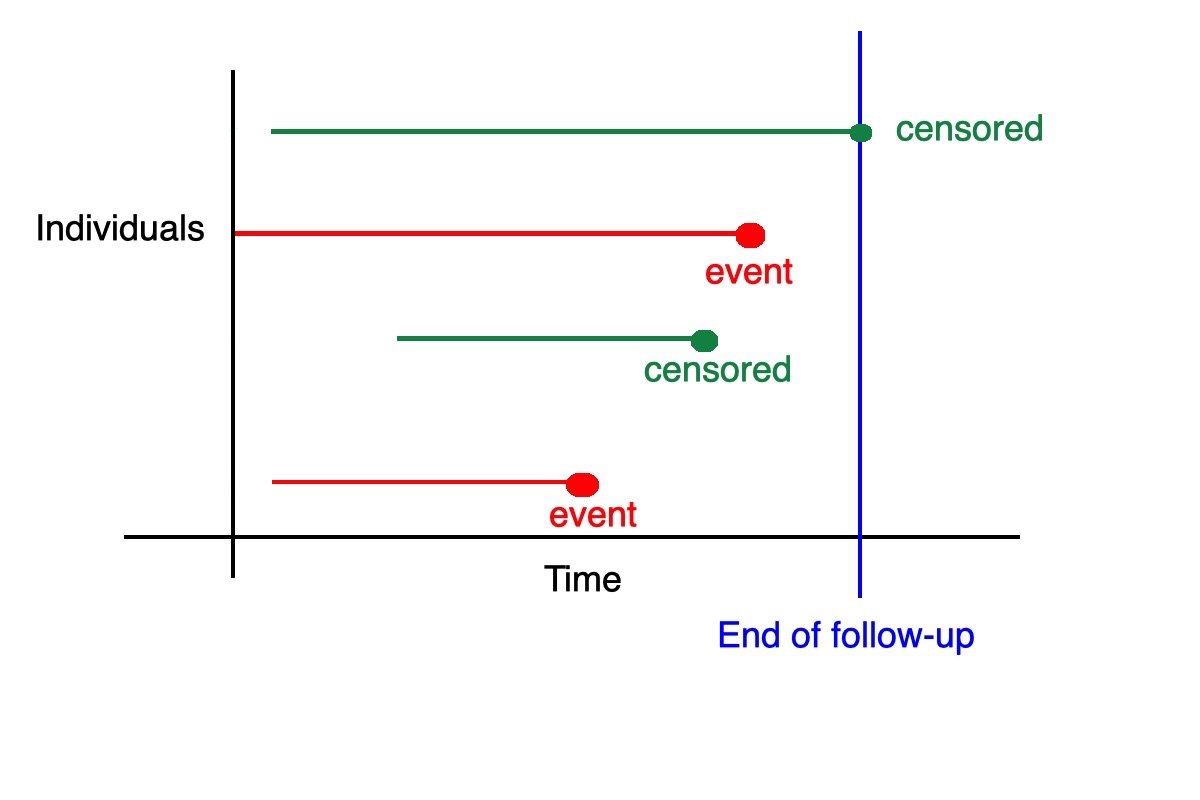
\includegraphics[scale=0.25]{censor}
\end{center}
\end{figure}
\end{frame}

\begin{frame}
\frametitle{Aims of Survival Analysis}
\begin{itemize}
\item One of the aims of Survival Analysis is to quantify the survival of the group of individuals. The typical quantities of interests are: \pause
\begin{enumerate}
\item The \textbf{survival function} $S(t) = 1- F(t) = \pr(T>t)$,  where $T$ is a positive random variable representing the survival time with CDF $F$.
\pause
\item The \textbf{hazard function} is defined as the instantaneous risk:
$$h(t) = \lim_{dt \to 0} \dfrac{P[t \leq  T < t+dt \mid  T \geq t]}{dt} \pause \stackrel{\tiny homework}{=} \dfrac{f(t)}{S(t)}.$$ 
\end{enumerate}
\end{itemize}
\end{frame}

\begin{frame}
\frametitle{Survival and Hazard functions}
\begin{itemize}
\item The hazard function and the survival function are linked through the relationship:
$$S(t) \stackrel{\tiny homework}{=} \exp\left\{ - \int_0^t h(s) ds \right\}.$$
\pause
\item The function $H(t) = \int_0^t h(s) ds$ is known as the \textbf{cumulative hazard} function.
\end{itemize}
\end{frame}

\begin{frame}
\frametitle{The importance of the hazard function}
\setbeamercovered{invisible}
\begin{itemize}
\item We are exposed to many forces of mortality: ageing, illnesses, natural disasters, accidents, crime, and etcetera.  

\pause

\item In Biostatistics (and epidemiology), the concept of the hazard plays a key role as it reflects these forces of mortality.
%\pause


%\item The mathematical definition of the hazard function appeared in the 1950s.

\end{itemize}
\end{frame}


\begin{frame}
\frametitle{Maximum Likelihood Estimation: No covariates}
\begin{itemize}
\item Suppose that $(t_1,\ldots,t_n)$ are independent and identically distributed.
\pause
\item Suppose that we are interested in estimating the survival function using a parametric distribution $F(\cdot \mid \btheta)$.
\pause
\item Which distribution?
\end{itemize}
\end{frame}



\begin{frame}
\frametitle{Brief catalogue of parametric distributions}
\begin{itemize}
\item \href{https://en.wikipedia.org/wiki/Gamma_distribution}{[Gamma]}.
\item \href{https://en.wikipedia.org/wiki/Weibull_distribution}{[Weibull]}.
\item \href{https://en.wikipedia.org/wiki/Log-normal_distribution}{[Lognormal]}.
\item \href{https://en.wikipedia.org/wiki/Log-logistic_distribution}{[Loglogistic]}.
\item \href{https://en.wikipedia.org/wiki/Generalized_gamma_distribution}{[Generalised Gamma]}.
\item Among many many others. \href{https://rpubs.com/FJRubio/PGW}{[see]}
\end{itemize}
\end{frame}

\begin{frame}
\frametitle{\textcolor{red}{Warning:}}
Different distributions can capture different shapes of the hazard function: \pause
\vspace{0.5cm}
\begin{itemize}
\item Weibull: increasing, decreasing, flat. \pause
\item Lognormal: unimodal (up then down). \pause
\item Generalised gamma:  increasing, decreasing, bathtub, and unimodal. \pause
\end{itemize}
\vspace{0.5cm}
By selecting a parametric from the catalogue of distributions, we are making assumptions about the possible hazard rates of the true distribution. Selecting the best model using formal tools is usually recommended.
\end{frame}


\begin{frame}
\frametitle{Maximum Likelihood Estimation: No covariates}
\begin{itemize}
\item We need to take the difference in the contribution of the \textcolor{blue}{observed} and \textcolor{red}{right-censored} times: \pause
\begin{eqnarray*}
L(\btheta) = \prod_{i=1}^n \textcolor{blue}{f(t_i \mid \btheta)^{\delta_i}} \textcolor{red}{S(t_i \mid \btheta)^{1-\delta_i}}.
\end{eqnarray*}
\pause
\item The MLE $\widehat{\btheta}$ of $\btheta$ is the value that maximises the likelihood function (numerical methods).
\pause
\item The fitted survival and hazard functions are  $S(t\mid \widehat{\btheta})$ and $h(t\mid \widehat{\btheta})$.
\end{itemize}
\end{frame}


\begin{frame}
\frametitle{Software}
\begin{itemize}
\item Since these are standard methods and distributions, many have already been implemented in R.
\pause
\item Fitting a number of distributions to survival data using the \href{https://cran.r-project.org/web/packages/flexsurv/vignettes/flexsurv.pdf}{[flexsurv]} R package.
\end{itemize}
\end{frame}


\begin{frame}
\frametitle{Regression models: using covariates}
\begin{itemize}
\item Spoiler: there is not unique way of including covariates to model survival times.
\pause
\item Biostatisticians and epidemiologists tend to think in terms of the hazard, based on the previous interpretation. \pause Thus, unsurprisingly, most approaches to include covariates in the survival model consist of hazard-based regression models.
\pause
\item The most popular models are: the proportional hazards (PH) model, and the accelerated failure time (AFT) model.
\end{itemize}
\end{frame}


\begin{frame}
\frametitle{Proportional hazards models}
\begin{itemize}
\item The PH model postulates that the covariates affect a ``baseline hazard'', by either increasing it  or decreasing it. This is,
\pause
\begin{equation*}
h_{PH}(t \mid \bx_i, \btheta,\bbeta) = h_0(t \mid \btheta) \exp\left\{ \bx_i ^{\top}\bbeta\right\} .
\end{equation*}
\pause
\item The corresponding cumulative hazard function is:
\begin{equation*}
H_{PH}(t \mid \bx_i, \btheta,\bbeta) \stackrel{\tiny homework}{=}  H_0(t \mid \btheta) \exp\left\{ \bx_i ^{\top}\bbeta\right\}.  
\end{equation*}
\end{itemize}
\end{frame}


\begin{frame}
\frametitle{Proportional hazards: interpretation}
\begin{itemize}
\item $h_0(t \mid \btheta)$ is the hazard associated to $\bx_i = {\bf 0}$. This represents a sort of ``reference point''. This can be the hazard associated to the distributions discussed previously.
\pause
\item If $\bx_i ^{\top}\bbeta >0$, 
\[h_{PH}(t \mid \bx_i, \btheta,\bbeta) > h_0(t \mid \btheta).\]
\pause This means that the combination of characteristics of the individual, for a fixed value of $\bbeta$, lead to an increase of the hazard compared to the baseline hazard. \pause
\item If $\bx_i ^{\top}\bbeta <0$, 
\[h_{PH}(t \mid \bx_i, \btheta,\bbeta) < h_0(t \mid \btheta).\]
\pause This means that the combination of characteristics of the individual, for a fixed value of $\bbeta$, lead to an decrease of the hazard compared to the baseline hazard.
\end{itemize}
\end{frame}


\begin{frame}
\frametitle{Proportional hazards: hazard ratios}
\begin{itemize}
\item Let $\bx_i$ denote the characteristics of the $i$th patient. \pause
\item For a specific value of $k\in\{1,\dots,p\}$, let $\tilde{\bx}_i$ be defined as 
\begin{eqnarray*}
\tilde{x}_{ij} =
\begin{cases}
x_{ij} & j\neq k,\\
x_{ij}+1 & j = k.
\end{cases}
\end{eqnarray*}
\pause
\item Then,
\[ \dfrac{h_{PH}(t \mid \tilde{\bx}_i, \btheta,\bbeta)}{h_{PH}(t \mid \bx_i, \btheta,\bbeta)}  \stackrel{\tiny homework}{=} \exp\{\bbeta_k\} .\]
\pause This is, the exponential of $\bbeta_k$ represents the increase in hazard due to an increase of one unit of the covariate  $x_{ik}$.
\end{itemize}
\end{frame}

\begin{frame}
\frametitle{Accelerated Failure Time model}
\begin{itemize}
\item The AFT postulates that covariates affect simultaneously the time scale and the hazard scale:
\begin{equation*}
h_{AFT}(t \mid \bx_i, \btheta,\bbeta) = h_0\left(t  \exp\left\{ \bx_i ^{\top}\bbeta\right\}\mid \btheta\right) \exp\left\{ \bx_i ^{\top}\bbeta\right\} .
\end{equation*}
\pause
\item The corresponding cumulative hazard function is:
\begin{equation*}
H_{AFT}(t \mid \bx_i, \btheta,\bbeta) \stackrel{\tiny homework}{=}  H_0\left(t  \exp\left\{ \bx_i ^{\top}\bbeta\right\}\mid \btheta\right)  .
\end{equation*}
\end{itemize}
\end{frame}

\begin{frame}
\frametitle{AFT model: interpretation}
\begin{itemize}
\item The interpretation of the AFT model is easier if we transform the model as follows. The survival function is:
\begin{eqnarray*}
S_{AFT}(t_i \mid \bx_i, \btheta,\bbeta) &\stackrel{\tiny homework}{=}& \exp \left\{- H_0\left(t_i  \exp\left\{ \bx_i ^{\top}\bbeta\right\}\mid \btheta\right) \right\} \\
 &=& S_0\left(t_i  \exp\left\{ \bx_i ^{\top}\bbeta\right\}\mid \btheta\right)\\
 &=& 1-F_0\left(t_i  \exp\left\{ \bx_i ^{\top}\bbeta\right\}\mid \btheta\right)\\
 &=& {\mathbb P}  \left( T_i > t_i  \exp\left\{ \bx_i ^{\top}\bbeta\right\}\mid \btheta\right)\\
 &=& {\mathbb P}  \left(\log T_i > \log(t_i)  + \bx_i ^{\top}\bbeta \mid \btheta\right)\\
 &=& {\mathbb P}  \left(\log T_i > \log(t_i)  - \bx_i ^{\top}\balpha \mid \btheta\right),
\end{eqnarray*}
where $\balpha = -\bbeta$.
\end{itemize}
\end{frame}

\begin{frame}
\frametitle{AFT model: interpretation}
\begin{itemize}
\item Let $Y_i = \log(T_i)$ and  $Y_i \mid   \bx_i ^{\top}\balpha  \sim G_0(\cdot \mid \btheta)$. Let $g_0$ be the corresponding pdf.
\pause 
\item  Then,
\begin{eqnarray*}
S_{AFT}(t_i \mid \bx_i, \btheta,\bbeta) \leftrightarrow 1-G_0\left( y_i   - \bx_i ^{\top}\balpha \mid \btheta\right).
\end{eqnarray*}
\pause
\item Consequently, the density function is 
\begin{eqnarray*}
f_{AFT}(t_i \mid \bx_i, \btheta,\bbeta) \leftrightarrow  g_0\left( y_i   - \bx_i^{\top}\balpha \mid \btheta\right).
\end{eqnarray*}
\pause
\item Finally, we can identify this pdf with the pdf associated to a log-linear model:
\begin{eqnarray*}
y_i = \log(t_i) =  \bx_i ^{\top}\balpha + \epsilon_i, \,\,\, i=1,\dots,n,
\end{eqnarray*}
where $\epsilon_i \stackrel{iid}{\sim} G_0(\cdot \mid \btheta)$. \pause
\item Consequently, the covariates have a direct effect on the log survival time.

\end{itemize}
\end{frame}



\begin{frame}
\frametitle{Regression models: the likelihood function}
\pause
\begin{itemize}
\item The likelihood function (for PH and AFT models) is:
\begin{eqnarray*}
L(\bbeta,\btheta) &=& \prod_{i=1}^n \textcolor{blue}{f_{j}(t_i \mid {\bx}_i, \btheta,\bbeta)^{\delta_i}} \textcolor{red}{S_{j}(t_i \mid {\bx}_i, \btheta,\bbeta)^{1-\delta_i}}\\
\pause  &\stackrel{\tiny homework}{=}& \prod_{i=1}^n h_{j}(t_i \mid {\bx}_i, \btheta,\bbeta)^{\delta_i} \exp\left\{ - H_{j}(t_i \mid {\bx}_i, \btheta,\bbeta) \right\},\,\,\, (*)
\end{eqnarray*} 
$j=PH,AFT$.

\item This also shows that the likelihood can be characterised using the hazard function.
\end{itemize}
\end{frame}

\begin{frame}
\frametitle{Example: lung cancer data}
\begin{itemize}
\item Let $t_i$, $i=1,\dots,228$ denote the survival times associated to patients with advanced lung cancer from the North Central Cancer Treatment Group.
\item 165 patients died within the follow-up period (1022 days).

\end{itemize}
\end{frame}


\begin{frame}
\frametitle{No covariates}
\begin{itemize}
\item In the first scenario, we compare the survival functions associated to three parametric models: Weibull, Lognormal, and Generalised Gamma. \pause R code \href{https://rpubs.com/FJRubio/PSM}{Example: no covariates}.

\end{itemize}
\end{frame}

\begin{frame}
\frametitle{Regression models}
\begin{itemize}
\item We consider two covariates, ``age'' and  ``sex'' . We first compare the PH and AFT models using a lognormal baseline hazard, and later a Weibull baseline hazard (where PH=AFT). \pause R code \href{https://rpubs.com/FJRubio/PSRM}{Example: Regression}.
\end{itemize}
\end{frame}


\begin{frame}
\frametitle{Discussion}
\begin{itemize}
\item Parametric survival models are useful tools in several applied areas.
\pause
\item Their use is not automatic as the user needs to select the parametric model(s).
\pause
\item PH and AFT models are the most popular hazard-based regression models.
\pause
\item Confidence intervals for the parameters and confidence regions for the estimate of the survival function.
\end{itemize}
\end{frame}

\begin{frame}
\frametitle{Extensions: Parametric approaches}
\begin{itemize}
\item The General Hazard (GH) model represents an extension of the PH and AFT models.
\item The GH model is discussed in Lecture II.
\item The GH model is implemented in the R package \href{https://github.com/FJRubio67/HazReg}{[HazReg]}.
\item Other model structures include the Proportional Odds model and related extensions.
\end{itemize}
\end{frame}

\begin{frame}
\frametitle{Extensions: Semiparametric and Nonparametric approaches}
\begin{itemize}
\item The Kaplan-Meier estimator is a NP estimator of the survival function.
\item The Nelson-Aalen estimator is a NP estimator of the cumulative hazard function.
\item The Cox model is a semiparametric version of the PH model.
\begin{center}
\url{https://rpubs.com/FJRubio/CPHM}
\end{center}

\end{itemize}
\end{frame}


\begin{frame}
\frametitle{The Cox PH Model and the Partial Likelihood function}
\begin{itemize}
\item The PH model:
$$
h_{PH}(t\mid \bx_i, \bbeta) = h_0(t)\exp\left\{\bx_i^{\top}\bbeta \right\},
$$
\pause
\item In order to avoid misspecification of the baseline hazard (wrong model), it is often preferred to estimate it non-parametrically, while the coefficients $\bbeta$ are estimated using the log partial likelihood function \cite{cox:1972}: \pause
$$
\ell_p(\bbeta) = \sum_{\delta_i=1} \bx_i^{\top}\bbeta  - \sum_{\delta_i=1} \log\left( \sum_{k \in {\mathcal R}(t_i)} \exp\left\{\bx_k^{\top}\bbeta\right\}\right),
$$
where $t_i$, $i=1,\dots,n$, are the survival times, ${\mathcal R}(t) = \{i : t_i \geq t\}$ denotes the risk set at time $t$.
\end{itemize}
\end{frame}


%\begin{frame}
%\frametitle{Extensions 2: Splines models}
%\begin{itemize}
%\item Typically including a model of the logarithm of the hazard function:
%\begin{eqnarray*}
%\log h(t) = g(t ; \bgamma),
%\end{eqnarray*}
%where is a spline basis expansion.
%\end{itemize}
%\end{frame}

\nocite{KP11} \nocite{klein:2016} \nocite{harrell:2015}

%\begin{frame}<beamer:0>
\bibliographystyle{plainnat}
\bibliography{references}
%\end{frame}
\end{document}
%
%





